% Course notes, part I: Model Predictive Control
% Process Identification and Control, 2026/2027 - Sapienza University of Rome, DIAG
\documentclass[11pt,a4paper]{article}

\usepackage[utf8]{inputenc}
\usepackage[T1]{fontenc}
\usepackage{lmodern}
\usepackage{microtype}
\usepackage[a4paper,margin=27mm,headheight=14pt]{geometry}
\usepackage{amsmath,amssymb,amsthm,mathtools}
\usepackage{booktabs}
\usepackage{enumitem}
\usepackage{xcolor}
\usepackage{tikz}
\usetikzlibrary{arrows.meta,positioning,calc,shapes.geometric,shapes.symbols,decorations.pathreplacing,patterns}
\usepackage[many]{tcolorbox}
\usepackage{caption}
\usepackage[hidelinks]{hyperref}
\usepackage{cleveref}

\definecolor{mpc}{RGB}{47,102,144}
\definecolor{sap}{RGB}{138,28,47}
\definecolor{ess}{RGB}{58,125,68}
\definecolor{sun}{RGB}{200,137,26}
\definecolor{soft}{RGB}{245,243,240}

\setlist{itemsep=2pt,topsep=3pt}
\captionsetup{font=small,labelfont=bf}

% ---- theorem-like environments -------------------------------------------
\theoremstyle{definition}
\newtheorem{definition}{Definition}[section]
\newtheorem{example}[definition]{Example}
\theoremstyle{plain}
\newtheorem{theorem}[definition]{Theorem}
\newtheorem{proposition}[definition]{Proposition}
\newtheorem{assumption}[definition]{Assumption}
\theoremstyle{remark}
\newtheorem{remark}[definition]{Remark}

% ---- boxes ----------------------------------------------------------------
\newtcolorbox{reading}{enhanced,breakable,colback=soft,colframe=sap,boxrule=0.6pt,
  arc=2pt,left=6pt,right=6pt,top=4pt,bottom=4pt,
  title=Further reading,fonttitle=\bfseries\small,coltitle=white,colbacktitle=sap}
\newtcolorbox{labbox}{enhanced,breakable,colback=soft,colframe=mpc,boxrule=0.6pt,
  arc=2pt,left=6pt,right=6pt,top=4pt,bottom=4pt,
  title=On the course website,fonttitle=\bfseries\small,coltitle=white,colbacktitle=mpc}
\newtcolorbox{keybox}{enhanced,breakable,colback=white,colframe=mpc,boxrule=0.8pt,
  arc=2pt,left=6pt,right=6pt,top=4pt,bottom=4pt}

% ---- notation -------------------------------------------------------------
\newcommand{\R}{\mathbb{R}}
\newcommand{\N}{\mathbb{N}}
\newcommand{\X}{\mathcal{X}}
\newcommand{\U}{\mathcal{U}}
\newcommand{\Xf}{\mathcal{X}_f}
\newcommand{\st}{\text{s.t.}\;}
\newcommand{\T}{^{\top}}
\newcommand{\norm}[1]{\left\lVert #1 \right\rVert}
\newcommand{\abs}[1]{\left\lvert #1 \right\rvert}
\newcommand{\bu}{\mathbf{u}}
\newcommand{\bx}{\mathbf{x}}
\newcommand{\ik}[1]{{#1|k}}
\DeclareMathOperator*{\argmin}{arg\,min}
\newcommand{\refkey}[1]{\textsf{[#1]}}

\title{\vspace{-8mm}\textbf{Model Predictive Control}\\[2mm]
  \large Course notes, part I\\[3mm]
  \normalsize Process Identification and Control, academic year 2026/2027\\
  Sapienza University of Rome, DIAG}
\author{}
\date{\small Version of 27 October 2026 --- to be completed after the lesson on task scheduling}

\begin{document}
\maketitle

\begin{center}
\begin{minipage}{0.9\textwidth}\small
These notes cover the first part of the course, on model predictive control. They follow the
route of the lessons, from the idea of the receding horizon to the theory of optimality,
feasibility and stability, and then to the case studies, but they are written to be read on their
own. Each chapter ends with the references for a deeper study; they are the same as those given
on the course website, with the same section and page numbers. The interactive laboratories
mentioned in the text are on the website, in the lesson diary.
\end{minipage}
\end{center}

\tableofcontents
\clearpage

\section{The receding-horizon idea}
\label{sec:intro}

\subsection{What a controller has to do}

A \emph{process} is a system whose evolution in time we want to influence: a tank whose
level has to be kept constant, a storage system whose charge has to follow the needs of a
building, a traffic light whose colours have to keep the queues short. We act on the process
through its \emph{control inputs} and we observe it through its \emph{measurements}. A
\emph{controller} is the rule that, at every sampling time, turns the measurements into the next
value of the inputs.

Classical controllers, such as the PID, compute the input from the current error with a fixed
formula. They are simple and robust, but they do not know the limits of the process --- a pump
that cannot exceed its rated power, a tank that cannot be emptied below a minimum level --- and
they do not look ahead. Model predictive control (MPC) is a different way of writing a controller:
at every sampling time it \emph{plans} the inputs over a window of future steps by solving an
optimization problem, and it uses only the first step of the plan.

\subsection{The receding horizon}

Fix a sampling time $T$ and call $k = 0, 1, 2, \dots$ the sampling instants. At time $k$ the
controller measures the state $x_k$ of the process, and considers the next $N$ steps, the
\emph{prediction horizon}. Inside the window it uses a second time index, $i = 0, 1, \dots, N$,
relative to the beginning of the window: the quantity predicted for step $i$ of the window opened
at time $k$ is written with the double index $i|k$, as in $x_{\ik{i}}$ and $u_{\ik{i}}$. The
absolute time of that step is $k + i$.

The controller then solves an optimization problem whose unknowns are the inputs over the
window, $u_{\ik{0}}, \dots, u_{\ik{N-1}}$, and whose cost measures how well the predicted
trajectory meets the control goal. Of the optimal sequence only the first element is applied to
the process, $u_k = u^*_{\ik{0}}$. At time $k+1$ the state is measured again and the whole
procedure is repeated over a window that has moved one step forward. This is the
\emph{receding horizon}: the window recedes as time advances (\cref{fig:receding}).

\begin{figure}[t]
\centering
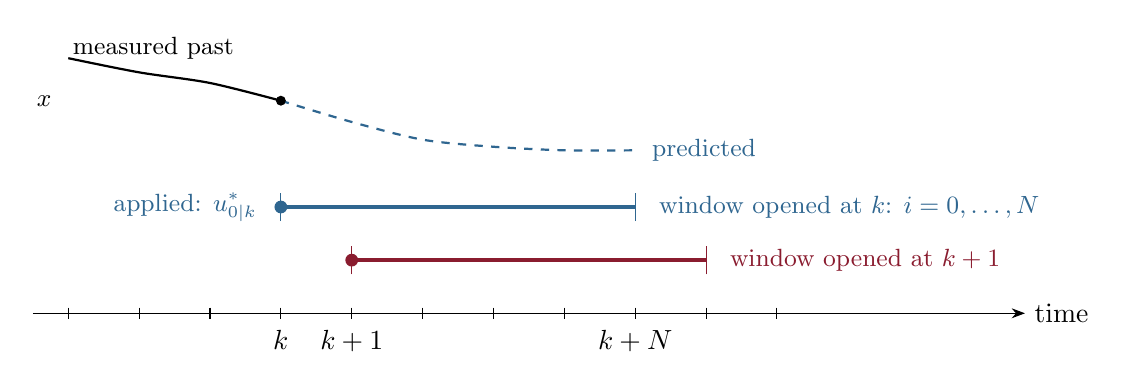
\begin{tikzpicture}[x=0.9cm,y=0.9cm,>=Stealth]
  % time axis
  \draw[->] (-0.5,0) -- (13.5,0) node[right] {time};
  \foreach \t in {0,...,10} \draw (\t,0.08) -- (\t,-0.08);
  \node[below] at (3,-0.1) {$k$};
  \node[below] at (4,-0.1) {$k+1$};
  \node[below] at (8,-0.1) {$k+N$};
  % window at k
  \draw[very thick,mpc] (3,1.5) -- (8,1.5);
  \draw[mpc] (3,1.3) -- (3,1.7);
  \draw[mpc] (8,1.3) -- (8,1.7);
  \node[right,mpc,font=\small] at (8.2,1.5) {window opened at $k$: $i = 0,\dots,N$};
  \fill[mpc] (3,1.5) circle (0.09);
  \node[left,mpc,font=\small] at (2.8,1.5) {applied: $u^*_{0|k}$};
  % window at k+1
  \draw[very thick,sap] (4,0.75) -- (9,0.75);
  \draw[sap] (4,0.55) -- (4,0.95);
  \draw[sap] (9,0.55) -- (9,0.95);
  \fill[sap] (4,0.75) circle (0.09);
  \node[right,sap,font=\small] at (9.2,0.75) {window opened at $k+1$};
  % predicted trajectory sketch
  \draw[thick,mpc,dashed] plot[smooth] coordinates {(3,3.0) (4,2.7) (5,2.45) (6,2.35) (7,2.3) (8,2.3)};
  \draw[thick] plot[smooth] coordinates {(0,3.6) (1,3.4) (2,3.25) (3,3.0)};
  \fill (3,3.0) circle (0.07);
  \node[above,font=\small] at (1.2,3.45) {measured past};
  \node[right,mpc,font=\small] at (8.1,2.3) {predicted};
  \node[left,font=\small] at (-0.1,3.0) {$x$};
\end{tikzpicture}
\caption{The receding horizon. At time $k$ the controller measures $x_k$, plans the inputs over
the next $N$ steps, applies the first one and discards the rest. At $k+1$ it starts again with a
window moved one step ahead.}
\label{fig:receding}
\end{figure}

\subsection{The nominal MPC algorithm}

The procedure can be written as an algorithm. The adjective \emph{nominal} means that the
controller trusts its model completely: no disturbances, no model errors, a state that can be
measured.

\begin{keybox}
\textbf{Nominal MPC.} At every sampling time $k$:
\begin{enumerate}[label=\arabic*.]
  \item measure the state $x_k$ of the process;
  \item solve the optimization problem $\mathcal{P}_N(x_k)$ over the window $i = 0,\dots,N$,
        obtaining the optimal input sequence $\bu^*_k = \{u^*_{\ik{0}},\dots,u^*_{\ik{N-1}}\}$;
  \item apply $u_k = u^*_{\ik{0}}$ to the process and discard the rest of the sequence;
  \item wait for the next sampling time and go back to step 1.
\end{enumerate}
\end{keybox}

The first input of the optimal sequence depends on the measured state: $u^*_{\ik{0}} =
\kappa_N(x_k)$. MPC is therefore a \emph{feedback} controller, not an open-loop plan computed
once, and $\kappa_N$ is its control law. It is a law that is never written down explicitly: it is
evaluated, at every step, by solving an optimization problem. This has two consequences that run
through the whole course. First, MPC is a nonlinear controller even when the process is linear,
because $\kappa_N$ is the solution of a constrained problem. Second, the time needed to solve the
problem must be much smaller than the sampling time $T$, which is the main practical limit of
the technique.

\subsection{Why MPC, and at what price}

The strength of MPC is that the goals of the control problem are written \emph{directly} into
the optimization problem: the cost says what we want, the constraints say what is admissible.
Limits on inputs and states --- the power of a pump, the capacity of a battery, the maximum
number of vehicles a queue can hold --- are constraints, not afterthoughts; several inputs and
several outputs are handled at once; and known information about the future, such as a forecast
of the demand or the schedule of a tariff, enters the plan naturally. The formulation is also
easy to explain to whoever operates the process, because every term has a meaning.

The price is twofold. The controller needs a \emph{model} of the process, good enough for its
predictions to be useful over the window; obtaining such a model is the subject of the third
part of the course. And it needs an optimization problem to be solved at every sampling time,
which rules out, or makes expensive, the cases in which the sampling time is very short or the
problem is very large.

The problems solved by MPC belong to two families. When all the decision variables are
continuous and the cost and the constraints are convex --- a quadratic cost with linear
constraints is the typical case --- the problem is a \emph{continuous program}, solved reliably
and fast. When some decisions are logical --- start a machine or not, turn a light green or
not --- they are represented by binary variables and the problem becomes a
\emph{mixed-integer program}, much harder in general. Both families appear in the case studies.

\subsection{Centralized and decentralized control}

When the process is made of many parts --- the intersections of a city, the buildings of a
district, the vehicles of a fleet --- one can write a single optimization problem for the whole
system, which is \emph{centralized} MPC, or one problem per part, each with its own controller,
which is \emph{decentralized} MPC; when the local controllers exchange information, the scheme
is called \emph{distributed}. The centralized problem is optimal but large; the local problems
are small but have to deal with the \emph{coupling constraints} that tie the parts together.
The case studies of this part are centralized; the question comes back with the aggregation of
electric vehicles and with the control of several intersections.

\subsection{Hard and soft constraints}

A constraint is \emph{hard} when it must hold without exception: the physical limit of an
actuator, the safety limit of a tank. It is \emph{soft} when it expresses a preference that may
be violated at a cost: a reference level, a deadline for a job. Soft constraints are written by
adding a non-negative \emph{slack} variable that measures the violation and by charging it in the
cost; \cref{sec:soft} shows the construction. The distinction matters because a problem whose
hard constraints cannot all be satisfied has no solution, and a controller with no solution has
nothing to apply.

\begin{reading}
\refkey{Rawlings\_2017}, sections 1.1 and 1.2 (pp.~1--10), for the setting of the problem and for
modelling; \refkey{Cannon\_2016}, chapter 1, for an overview of predictive control. The slides on
MPC of the course website, up to slide 25, cover this chapter.
\end{reading}

\section{Models and the optimization problem of MPC}
\label{sec:problem}

\subsection{State-space models}

A \emph{dynamical system} is described by a set of \emph{state variables}, collected in the state
vector $x \in \R^n$, which summarize its past: given the state at one instant and the inputs from
then on, the future of the system is determined. The inputs are collected in $u \in \R^m$, the
measured outputs in $y \in \R^p$.

In continuous time the model is a differential equation, $\dot x(t) = f_c(x(t), u(t))$. The
controller, however, acts at the sampling instants, so the model it uses is in discrete time:
\begin{equation}
  x_{k+1} = f(x_k, u_k), \qquad y_k = h(x_k).
  \label{eq:model}
\end{equation}
The model is \emph{linear} when $f(x,u) = Ax + Bu$ and $h(x) = Cx$ for constant matrices $A$,
$B$, $C$; it is \emph{nonlinear} otherwise. Three examples were worked out in class: a mass
connected to a spring and a damper and pushed by a force, whose state is the pair (position,
velocity) and whose model is linear; a pendulum driven by a torque, nonlinear because of the
gravitational term $\sin\theta$; an RLC circuit, linear. The procedure is always the same: write
the physical balance equations, choose the states, the inputs and the outputs, and rewrite the
equations in the form \eqref{eq:model}.

An \emph{equilibrium} of \eqref{eq:model} under a constant input $\bar u$ is a state $x^{eq}$
that the system does not leave, $x^{eq} = f(x^{eq}, \bar u)$. A system may have one, several or
infinitely many equilibria, or none: the pendulum has two families of them, the hanging and the
upright position repeated at every full turn. Without loss of generality the equilibrium of
interest is placed at the origin, $f(0,0) = 0$, by a change of variables.

\subsection{The problem solved at every step}

The optimization problem that MPC solves at time $k$, from the measured state $x_k$, is
\begin{equation}
\begin{aligned}
  \mathcal{P}_N(x_k):\quad
  \min_{u_{\ik{0}},\dots,u_{\ik{N-1}}} \quad
    & V_N(x_k, \bu_k) = \sum_{i=0}^{N-1} \ell\big(x_{\ik{i}}, u_{\ik{i}}\big) + V_f\big(x_{\ik{N}}\big) \\
  \st \quad
    & x_{\ik{i+1}} = f(x_{\ik{i}}, u_{\ik{i}}), \qquad i = 0,\dots,N-1, \\
    & x_{\ik{0}} = x_k, \\
    & u_{\ik{i}} \in \U, \qquad i = 0,\dots,N-1, \\
    & x_{\ik{i}} \in \X, \qquad i = 0,\dots,N, \\
    & x_{\ik{N}} \in \Xf .
\end{aligned}
\label{eq:PN}
\end{equation}
Its ingredients are the following.
\begin{itemize}
  \item The \emph{horizon} $N$: the number of steps the controller looks ahead. A longer horizon
        gives a better plan at the price of a larger problem.
  \item The \emph{stage cost} $\ell(x,u)$: the cost paid at each step, which encodes the goal.
        For a regulation problem, where the state has to be brought to the origin, the usual
        choice is quadratic,
        \begin{equation}
          \ell(x,u) = x\T Q x + u\T R u,
          \label{eq:quadcost}
        \end{equation}
        with $R$ positive definite and $Q$ positive definite, or positive semi-definite when only
        some of the states are penalized.
  \item The \emph{terminal cost} $V_f(x)$: the cost charged on the last predicted state. Its role,
        which is central, is the subject of \cref{sec:optimality}.
  \item The \emph{dynamics} as equality constraints, with the measured state as initial condition:
        this is where the model enters, and what makes the controller a feedback.
  \item The sets $\U$ and $\X$ of admissible inputs and states: the limits of the process. The
        common case is a box, $u^{\min} \le u \le u^{\max}$, $x^{\min} \le x \le x^{\max}$.
  \item The \emph{terminal set} $\Xf$, a constraint on the last predicted state. It is not
        required by the application: it is added to guarantee that the problem remains solvable
        from one step to the next, as \cref{sec:feasibility} explains.
\end{itemize}
The optimal value of the problem is written $V_N^*(x_k)$, and the first element of the optimal
sequence defines the control law, $\kappa_N(x_k) = u^*_{\ik{0}}$.

\begin{example}[the tank]
A tank of water volume $x$ is filled by a pump of power $u$ and emptied by a known consumption
$w$. With a sampling time $T$, the volume evolves as $x_{k+1} = x_k + a\,u_k - b\,w_k$. The
volume has to stay between a minimum and a maximum, the pump between zero and its rated power,
and the level has to be kept close to a reference $x^{ref}$. The problem solved at every step is
\eqref{eq:PN} with $\ell(x,u) = (x - x^{ref})^2 + \rho\,u^2$, box constraints on $x$ and $u$, and
no terminal set. Because the model is linear and the cost quadratic, $\mathcal{P}_N(x_k)$ is a
quadratic program. The Tank Control Lab on the course website runs this controller next to a
PID on the same tank: the PID has no knowledge of the limits and of the future consumption,
and the difference is visible in the volume trajectory and in the number of minutes spent
outside the admissible band.
\end{example}

\subsection{The ideal problem: infinite horizon}

Behind \eqref{eq:PN} there is the problem one would really like to solve, the
\emph{infinite-horizon constrained optimal control problem}:
\begin{equation}
  \min_{u_0,u_1,\dots}\ \sum_{i=0}^{\infty} \ell(x_i, u_i)
  \quad \st\quad x_{i+1} = f(x_i,u_i),\ x_0 = x_k,\ u_i \in \U,\ x_i \in \X .
  \label{eq:infhor}
\end{equation}
It has infinitely many variables and constraints, and in general it cannot be solved. With a
linear model and the quadratic cost \eqref{eq:quadcost} it is the \emph{constrained LQR}
problem, still out of reach because of the constraints.

The one case that can be solved exactly is the \emph{unconstrained} linear-quadratic problem.
Its solution is a linear state feedback, $u^*_k = K x_k$, with the gain $K$ given by the
discrete-time Riccati equation, and the closed-loop cost from any initial state is a quadratic
form:
\begin{equation}
  J^*(x_0) = \sum_{k=0}^{\infty}\big(x_k\T Q x_k + u_k\T R u_k\big) = x_0\T W x_0 ,
  \label{eq:Wcost}
\end{equation}
where $W$ solves the Lyapunov equation of the closed loop. The derivation is short: under the
law $u = Kx$ the state is $x_k = (A+BK)^k x_0$, the input $u_k = K(A+BK)^k x_0$, and
substituting both in the sum collapses it into a single quadratic form in $x_0$. The matrix $W$
is the quantity that does all the work in the next chapter.

\begin{reading}
\refkey{Cannon\_2016}, section 2.1, ``Problem Description'' (pp.~13--15): the same problem and
the same notation as in these notes; section 2.2, ``The Unconstrained Optimum'' (pp.~15--18):
the cost under a linear feedback, the Lyapunov equation for $W$ and the Riccati equation for
the gain. \refkey{Rawlings\_2017}, section 2.2, ``Model Predictive Control'' (pp.~91--106), for
the general formulation with stage cost, terminal cost and terminal set, and section 1.2,
``Models and Modeling'' (pp.~1--10), for the modelling part.
\end{reading}

\section{Optimality: a finite window for an infinite problem}
\label{sec:optimality}

This chapter answers one question: in what sense is the finite-horizon problem
$\mathcal{P}_N(x_k)$ a substitute for the infinite-horizon problem \eqref{eq:infhor}? The answer
goes through the value function and the principle of optimality, and it identifies the terminal
cost $V_f$ as the ingredient that makes the substitution exact. Throughout the chapter three
assumptions hold: the model is known and perfect, the state is measured, there are no
disturbances.

\subsection{The value function and Bellman's principle}

\begin{definition}[value function]
The \emph{value function} $V(x)$ is the optimal cost of the infinite-horizon problem
\eqref{eq:infhor} started at $x$: the cost of controlling the system optimally from $x$ onwards.
It is $+\infty$ when no admissible input sequence exists from $x$.
\end{definition}

\begin{theorem}[principle of optimality]
Let $\{u^*_0, u^*_1, \dots\}$ be an optimal input sequence for the problem started at $x_0$, and
let $x^*_N$ be the state it reaches at time $N$. Then the tail $\{u^*_N, u^*_{N+1}, \dots\}$ is an
optimal input sequence for the problem started at $x^*_N$.
\end{theorem}

The reason is simple: if a cheaper tail existed from $x^*_N$, replacing the tail of the original
sequence with it would give a cheaper sequence from $x_0$, against the optimality of the
original. The consequence is a decomposition of the optimal cost at any junction time $N$:
\begin{equation}
  V(x_0) = \sum_{i=0}^{N-1} \ell(x^*_i, u^*_i) + V(x^*_N).
  \label{eq:bellman}
\end{equation}
The optimal cost from $x_0$ is the cost of the first $N$ steps plus the value function of the
state reached: the infinite tail is summarized by one number.

\subsection{Dual-mode control}

Consider the constrained linear-quadratic problem. Assume the system controllable and the origin
strictly inside $\X$ and $\U$. Then an optimal sequence exists and its cost is finite; a finite
sum of positive-definite terms forces $x_k \to 0$ and $u_k \to 0$, so the constraints can be
active only in an initial phase. After some finite time $N$ the state is close enough to the
origin that the trajectory generated by the unconstrained law $u = Kx$ respects all the
constraints from then on, and by the principle of optimality applied to the tail problem that
law is not only admissible there, it is \emph{optimal}, because from that point on the
constrained and the unconstrained problems have the same solution.

This is \emph{dual-mode control}: the input is free in the first $N$ steps, and it is the LQR
feedback afterwards (\cref{fig:dualmode}). The tail is then known in closed form, and so is its
cost, $x_N\T W x_N$ from \eqref{eq:Wcost}. Substituting it in \eqref{eq:bellman}, the infinite
problem becomes
\begin{equation}
  \min_{u_0,\dots,u_{N-1}} \ \sum_{i=0}^{N-1}\big(x_i\T Q x_i + u_i\T R u_i\big) + x_N\T W x_N,
  \label{eq:dualmode}
\end{equation}
subject to the dynamics and the constraints over the first $N$ steps. This problem has $N$
decision variables and it is solvable. Its solution coincides with the first $N$ inputs of the
infinite-horizon optimum, $u^{*N}_k = u^{*\infty}_k$ for $k = 0,\dots,N-1$, provided $N$ is
large enough for the tail to be unconstrained.

\begin{figure}[t]
\centering
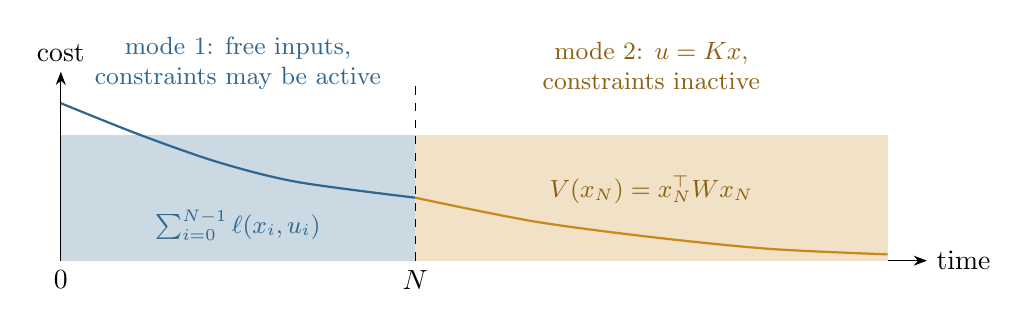
\begin{tikzpicture}[x=1cm,y=1cm,>=Stealth]
  \draw[->] (0,0) -- (11,0) node[right] {time};
  \draw[->] (0,0) -- (0,2.4) node[above] {cost};
  % first phase: free moves
  \fill[mpc!25] (0,0) rectangle (4.5,1.6);
  \draw[thick,mpc] plot[smooth] coordinates {(0,2.0) (1,1.6) (2,1.25) (3,1.0) (4.5,0.8)};
  \node[mpc,font=\small] at (2.25,0.45) {$\sum_{i=0}^{N-1}\ell(x_i,u_i)$};
  \node[mpc,font=\small,above,align=center] at (2.25,2.05) {mode 1: free inputs,\\constraints may be active};
  % tail
  \fill[sun!25] (4.5,0) rectangle (10.5,1.6);
  \draw[thick,sun] plot[smooth] coordinates {(4.5,0.8) (6,0.5) (7.5,0.3) (9,0.15) (10.5,0.08)};
  \node[sun!70!black,font=\small] at (7.5,0.9) {$V(x_N) = x_N\T W x_N$};
  \node[sun!70!black,font=\small,above,align=center] at (7.5,2.05) {mode 2: $u = Kx$,\\constraints inactive};
  \draw[dashed] (4.5,0) -- (4.5,2.3);
  \node[below] at (4.5,0) {$N$};
  \node[below] at (0,0) {$0$};
\end{tikzpicture}
\caption{Dual-mode control. In the first $N$ steps the inputs are free and the constraints may
be active; from $N$ on the unconstrained LQR feedback is optimal, and the cost of that tail is
the quadratic form $x_N\T W x_N$, which becomes the terminal cost of a finite-horizon problem.}
\label{fig:dualmode}
\end{figure}

\subsection{The terminal cost as the cost-to-go}

Problem \eqref{eq:dualmode} is $\mathcal{P}_N(x_k)$ with the quadratic stage cost and with
terminal cost $V_f(x) = x\T W x$. The lesson of the construction is general: the terminal cost
of an MPC problem should be the \emph{value function} of the infinite-horizon problem, the cost
of what happens after the window. When it is, the finite problem and the infinite one have the
same solution, and solving the finite problem again at every sampling time --- which is MPC ---
reproduces the infinite-horizon optimum. This is the precise sense in which MPC is optimal.

The practical difficulty is that $V(x)$ is unknown in general. The unconstrained
linear-quadratic problem is the exception: there $V(x) = x\T W x$ exactly, and this is why, in
linear-quadratic MPC, the terminal cost is taken from the Riccati or the Lyapunov equation and
the horizon is taken long enough. In other problems $V(x)$ has to be approximated, or learned:
the value function is also the object computed by dynamic programming, and learning it from
experience is the subject of reinforcement learning, the second part of the course.

\begin{remark}[the terminal weight matters]
The Service Area Lab on the website shows what happens when the terminal cost is not the value
function. With a window of twenty minutes and a terminal weight equal to the stage weight on the
stored energy, the controller is myopic: it sees almost no value in the state it leaves at the
end of the window, and the storage drifts away from its reference. With the terminal weight
from the Riccati equation, about four hundred times larger, the same twenty-minute controller
behaves like the infinite-horizon one.
\end{remark}

\subsection{From one step to the next}

Under the nominal assumptions, re-solving the problem at time $k+1$ returns the plan the
controller already had: $u^*_{\ik{1}}$ becomes $u^*_{0|k+1}$, and so on. The controller
confirms itself, and the receding horizon changes nothing. In reality the model is not perfect,
the forecasts are wrong and disturbances act on the process, so the state measured at $k+1$ is
not the one predicted; this is why the plan is rebuilt at every step rather than computed once.

The cost actually paid by the controller in closed loop is the sum of the stage costs along
the trajectory it generates, $J^{cl}(x_0) = \sum_{k \ge 0} \ell(x_k, \kappa_N(x_k))$. Its
difference from $V(x_0)$ is the \emph{optimality gap}; it is zero in the ideal conditions of
this chapter, and it measures what is lost when they fail.

\begin{reading}
\refkey{Cannon\_2016}, section 2.3, ``The Dual-Mode Prediction Paradigm'' (pp.~18--21);
Theorem~2.2 there is the formal version of the result of this chapter. \refkey{Rawlings\_2017},
sections 1.3.3 and 1.3.4 (pp.~18--23) and section 2.3, ``Dynamic Programming Solution''
(pp.~107--112), for the same material reached through dynamic programming, which is the road
taken again in the reinforcement learning part. Studying the proofs is optional.
\end{reading}

\section{Recursive feasibility}
\label{sec:feasibility}

A controller that applies the first step of a plan needs a plan at every step. If the
optimization problem has no admissible solution at some time $k$, the controller has nothing
to apply. The property that rules this out is the subject of this chapter.

\subsection{Feasible sets and invariance}

\begin{definition}[feasible set]
The \emph{feasible set} $\mathcal{F}_N$ of problem \eqref{eq:PN} is the set of states $x$ from
which the problem admits at least one admissible input sequence.
\end{definition}

\begin{definition}[recursive feasibility]
The MPC algorithm is \emph{recursively feasible} if, whenever $\mathcal{P}_N(x_k)$ has a solution,
$\mathcal{P}_N(x_{k+1})$ has a solution as well, with $x_{k+1} = f(x_k, \kappa_N(x_k))$. In
words: feasible once, feasible forever.
\end{definition}

Recursive feasibility is a statement about sets. For an autonomous system $x_{k+1} = g(x_k)$ a
set $S$ is \emph{positively invariant} when every state in $S$ is mapped into $S$: $x \in S
\Rightarrow g(x) \in S$. For a controlled system $x_{k+1} = f(x_k,u_k)$ a set $S$ is
\emph{controlled invariant} when for every $x \in S$ there exists an admissible input $u \in \U$
such that $f(x,u) \in S$. Recursive feasibility is exactly the statement that the MPC law makes
the feasible set controlled invariant: from every state in $\mathcal{F}_N$, the input it chooses
leads to a state that is again in $\mathcal{F}_N$ (\cref{fig:invariant}).

\begin{figure}[t]
\centering
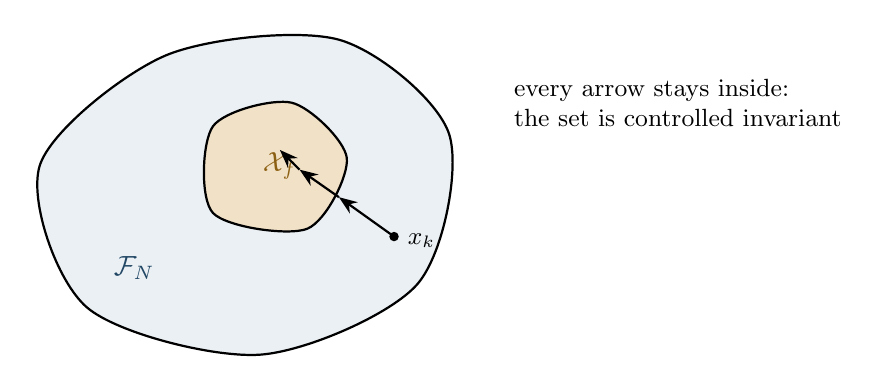
\begin{tikzpicture}[x=1cm,y=1cm,>=Stealth]
  \draw[thick,fill=mpc!10] plot[smooth cycle] coordinates {(0,0) (2.2,-0.6) (4.2,0.3) (4.6,2.2) (3.2,3.4) (1.0,3.2) (-0.6,1.8)};
  \draw[thick,fill=sun!25] plot[smooth cycle] coordinates {(1.6,1.2) (2.8,1.0) (3.3,1.9) (2.6,2.6) (1.6,2.3)};
  \node[mpc!70!black] at (0.6,0.5) {$\mathcal{F}_N$};
  \node[sun!70!black] at (2.45,1.8) {$\Xf$};
  % trajectory staying inside
  \fill (3.9,0.9) circle (0.06);
  \draw[->,thick] (3.9,0.9) -- (3.2,1.4);
  \draw[->,thick] (3.2,1.4) -- (2.7,1.75);
  \draw[->,thick] (2.7,1.75) -- (2.45,2.0);
  \node[right,font=\small] at (3.95,0.85) {$x_k$};
  \node[font=\small,align=left,anchor=west] at (5.3,2.6) {every arrow stays inside:\\the set is controlled invariant};
\end{tikzpicture}
\caption{The feasible set $\mathcal{F}_N$ and the terminal set $\Xf$. Recursive feasibility
means that the control law never takes the state out of $\mathcal{F}_N$; the terminal set is
the smaller set, controlled invariant under the terminal law, that makes the proof work.}
\label{fig:invariant}
\end{figure}

\subsection{The proof}

The proof is constructive, and the construction is the natural one. Assume the nominal
conditions, so that the state at $k+1$ is exactly the one the controller predicted,
$x_{k+1} = x^*_{\ik{1}}$. At time $k$ the controller found the optimal sequence
$\{u^*_{\ik{0}}, u^*_{\ik{1}}, \dots, u^*_{\ik{N-1}}\}$ with predicted states
$\{x^*_{\ik{0}}, \dots, x^*_{\ik{N}}\}$, and $x^*_{\ik{N}} \in \Xf$. At time $k+1$ build the
\emph{tentative} sequence
\begin{equation}
  \tilde\bu_{k+1} = \{\,u^*_{\ik{1}},\, u^*_{\ik{2}},\, \dots,\, u^*_{\ik{N-1}},\,
  \kappa_f(x^*_{\ik{N}})\,\},
  \label{eq:tail}
\end{equation}
the tail of the previous optimal sequence, completed with one more input given by a
\emph{terminal control law} $\kappa_f$ applied to the previous terminal state. The first $N-1$
inputs are admissible and produce admissible states, because they did so at time $k$ --- the
window has merely moved. Two things remain to be checked: that the appended input is
admissible, $\kappa_f(x^*_{\ik{N}}) \in \U$, and that the state it produces satisfies the
terminal constraint, $f\big(x^*_{\ik{N}}, \kappa_f(x^*_{\ik{N}})\big) \in \Xf$.

Both hold at once if the terminal set and the terminal law are chosen so that
\begin{equation}
  x \in \Xf \ \Rightarrow\ \kappa_f(x) \in \U \ \text{ and }\ f\big(x,\kappa_f(x)\big) \in \Xf ,
  \label{eq:terminalinv}
\end{equation}
that is, if $\kappa_f$ makes $\Xf$ positively invariant for the controlled system while
respecting the input constraints. Then \eqref{eq:tail} is an admissible sequence for
$\mathcal{P}_N(x_{k+1})$, the problem has at least one solution, and recursive feasibility
follows.

\begin{theorem}[recursive feasibility]
Under the nominal assumptions, if $\Xf$ and $\kappa_f$ satisfy \eqref{eq:terminalinv}, then
$\mathcal{P}_N(x_k)$ feasible implies $\mathcal{P}_N(x_{k+1})$ feasible, and the feasible set
$\mathcal{F}_N$ is controlled invariant under the MPC law.
\end{theorem}

\subsection{Choosing the terminal set}

Two examples of terminal law appeared in class. The law that does nothing, $\kappa_f(x) = 0$,
works when $\Xf$ is invariant for the uncontrolled system. The linear law $\kappa_f(x) = Kx$,
with $K$ the LQR gain, is the one that connects back to dual-mode control: $\Xf$ is then a set
inside which the unconstrained feedback respects all the constraints, and the second mode of
\cref{fig:dualmode} is exactly the terminal law.

The choice involves a trade-off. The terminal constraint $x_{\ik{N}} \in \Xf$ is \emph{added}
to the problem; it is not required by the application, and like every constraint it can only
make the optimal cost worse. A larger terminal set therefore means a larger feasible set and a
lower cost, and one looks for the largest $\Xf$ that admits a law satisfying
\eqref{eq:terminalinv}. Under that condition the feasible sets also grow with the horizon:
$\mathcal{F}_N \subseteq \mathcal{F}_{N+1}$, because a sequence that reaches $\Xf$ in $N$ steps,
extended with one step of the terminal law, reaches it in $N+1$.

\begin{remark}[when feasibility fails]
The Building Energy Lab on the website makes the failure visible: lower the contractual power
limit while forcing several appliances into the same narrow window, and the optimizer reports
that no admissible plan exists. The constraints are contradictory; the algorithm is not at
fault. The remedy, when the application allows it, is to make the constraints that may fail
soft, as in \cref{sec:soft}.
\end{remark}

\begin{reading}
\refkey{Cannon\_2016}, section 2.4, ``Invariant Sets'' (pp.~21--24), and section 2.5,
``Controlled Invariant Sets and Recursive Feasibility'' (pp.~24--29): the proof above in the
same form, with the nested feasible sets. \refkey{Rawlings\_2017}, section 2.4.2,
``Stabilizing Conditions'' (pp.~114--120), for the assumptions on the terminal set in their
standard form, and section 2.6, ``Is a Terminal Constraint Set Necessary?'' (pp.~144--147), for
what happens without one.
\end{reading}

\section{Stability}
\label{sec:stability}

Stability is a property of the equilibrium points of a dynamical system, not of the system as a
whole. Adding a feedback law turns the controlled system $x_{k+1} = f(x_k, u_k)$ into the
autonomous system $x_{k+1} = f(x_k, \kappa(x_k)) = \tilde f(x_k)$, and two questions arise: can
an unstable equilibrium be made stable by the controller, and can an equilibrium that was
stable be made unstable by it? For MPC the second question is the one that needs an answer,
because $\kappa_N$ is a nonlinear law that no classical criterion covers.

\subsection{Definitions}

Consider an autonomous system $x_{k+1} = \tilde f(x_k)$ with an equilibrium at the origin,
$\tilde f(0) = 0$.

\begin{definition}[stability]
The origin is \emph{stable} if for every $\varepsilon > 0$ there exists $\delta(\varepsilon) > 0$
such that $\norm{x_{k_0}} \le \delta$ implies $\norm{x_k} \le \varepsilon$ for all $k \ge k_0$.
It is \emph{asymptotically stable} if it is stable and, in addition, $x_k \to 0$ for every
initial state in some neighbourhood of the origin, the \emph{region of attraction}. It is
\emph{globally asymptotically stable} if the region of attraction is the whole state space.
\end{definition}

Stability says that small initial perturbations produce trajectories that remain forever close
(\cref{fig:epsdelta}); asymptotic stability adds that they return. Both are local notions
unless stated otherwise.

\begin{figure}[t]
\centering
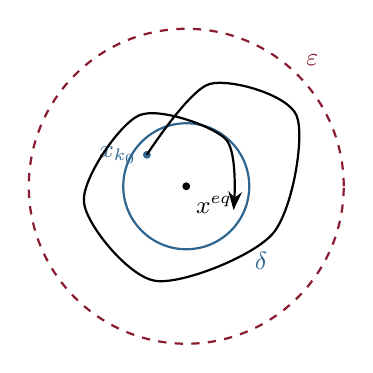
\begin{tikzpicture}[x=1cm,y=1cm,>=Stealth]
  \draw[thick,sap,dashed] (0,0) circle (2.0);
  \draw[thick,mpc] (0,0) circle (0.8);
  \fill (0,0) circle (0.05);
  \node[below right,font=\small] at (0,0) {$x^{eq}$};
  \node[mpc,font=\small] at (0.95,-0.95) {$\delta$};
  \node[sap,font=\small] at (1.6,1.6) {$\varepsilon$};
  \fill[mpc] (-0.5,0.4) circle (0.05);
  \node[mpc,font=\small,left] at (-0.5,0.4) {$x_{k_0}$};
  \draw[thick,->] plot[smooth] coordinates {(-0.5,0.4) (0.3,1.3) (1.4,0.9) (1.1,-0.6) (-0.4,-1.2) (-1.3,-0.2) (-0.6,0.9) (0.5,0.6) (0.6,-0.3)};
\end{tikzpicture}
\caption{The $\varepsilon$--$\delta$ definition of stability: a trajectory that starts within
$\delta$ of the equilibrium never leaves the ball of radius $\varepsilon$.}
\label{fig:epsdelta}
\end{figure}

\subsection{Linear systems}

For $x_{k+1} = A x_k$ the answer is complete. The solution is $x_k = A^k x_0$, and everything
depends on the eigenvalues of $A$: the origin is asymptotically stable if and only if all the
eigenvalues lie strictly inside the unit circle; it is unstable if at least one lies outside;
eigenvalues on the circle give simple stability when they are simple, and need a separate check
when they are repeated. This criterion is not enough for MPC: the model may be nonlinear, and
even for a linear model the controller $\kappa_N$ is nonlinear.

\subsection{Lyapunov functions}

\begin{definition}[definite functions]
A scalar function of the state $V: \R^n \to \R$ is \emph{positive definite} if $V(0) = 0$ and
$V(x) > 0$ for every $x \ne 0$; it is \emph{positive semi-definite} if $V(0) = 0$ and $V(x) \ge
0$ for every $x$. It is negative definite, or semi-definite, when $-V$ is positive definite, or
semi-definite. The \emph{local} versions of these definitions require the inequalities only in a
neighbourhood of the equilibrium.
\end{definition}

The quadratic forms $V(x) = x\T P x$ are the standard example: such a form is positive definite
if and only if all the eigenvalues of $P$ are positive. Not every candidate works: $V(x) =
2\sin^2(x_1) + 3x_2^2$ is positive definite only locally, since it vanishes at $(\pi, 0)$. The level sets
$\Omega_c = \{x : V(x) = c\}$ of a positive definite function are closed curves around the
origin, nested as $c$ grows; they are the geometric picture behind the theorems that follow.

The \emph{increment} of $V$ along the trajectories of the system is
\begin{equation}
  \Delta V(x) = V\big(\tilde f(x)\big) - V(x),
\end{equation}
the change of $V$ from one state to the next. It is computed along the trajectories, not in an
arbitrary direction.

\begin{theorem}[Lyapunov]
Let the origin be an equilibrium of $x_{k+1} = \tilde f(x_k)$. If there exists a continuous
function $V$, positive definite at least locally around the origin, such that $\Delta V$ is negative
semi-definite at least locally, then the origin is stable. If, in addition, $\Delta V$ is
negative definite, then the origin is asymptotically stable.
\end{theorem}

The condition $\Delta V \le 0$ is often written as $\Delta V(x) \le -h(x)$ with $h \ge 0$,
which says \emph{how much} $V$ must decrease at each step; this form is the one used in the
next section. The intuition is in \cref{fig:lyapunov}: if $V$ is positive and decreases along
the trajectory, the trajectory is confined to level sets of smaller and smaller value, and if
the decrease is strict then $V \to 0$ and with it $x_k \to 0$. A function tried as a candidate is
a \emph{candidate Lyapunov function}; one that satisfies both conditions is a \emph{Lyapunov
function}. The theorem is a sufficient condition: failing to find a Lyapunov function proves
nothing.

\begin{figure}[t]
\centering
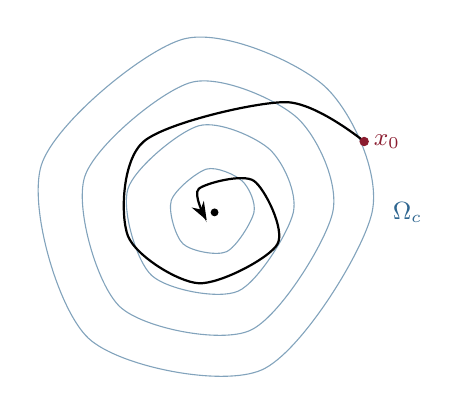
\begin{tikzpicture}[x=1cm,y=1cm,>=Stealth]
  \foreach \r in {0.5,1.0,1.5,2.0} {
    \draw[mpc!60] plot[smooth cycle] coordinates {(\r,0) (0.7*\r,0.8*\r) (-0.2*\r,1.1*\r) (-1.1*\r,0.3*\r) (-0.8*\r,-0.8*\r) (0.3*\r,-1.0*\r)};
  }
  \node[mpc,font=\small] at (2.45,0.0) {$\Omega_{c}$};
  \fill (0,0) circle (0.05);
  \draw[thick,->] plot[smooth] coordinates {(1.9,0.9) (0.9,1.4) (-0.9,0.9) (-1.1,-0.3) (-0.2,-0.9) (0.8,-0.4) (0.5,0.4) (-0.2,0.3) (-0.1,-0.1)};
  \fill[sap] (1.9,0.9) circle (0.06);
  \node[sap,font=\small,right] at (1.9,0.9) {$x_0$};
\end{tikzpicture}
\caption{Level sets of a positive definite function and a trajectory along which $V$ decreases
at every step: each level set traps the trajectory inside a smaller one.}
\label{fig:lyapunov}
\end{figure}

\subsection{Stability of MPC}

Take the regulation problem: the system has an equilibrium at the origin, $f(0,0) = 0$, the
stage cost $\ell(x,u)$ is positive definite in $(x,u)$, and the terminal cost $V_f(x)$ is
positive definite in $x$. These assumptions are satisfied by any reasonable regulation cost,
such as \eqref{eq:quadcost} with $Q$ and $R$ positive definite.

\paragraph{The equilibrium survives.} The closed loop is $x_{k+1} = f(x_k, \kappa_N(x_k)) =
\tilde f(x_k)$, so the origin is an equilibrium of $\tilde f$ if and only if $\kappa_N(0) = 0$. It
is: from $x_k = 0$ the sequence of all zeros is admissible, keeps the state at zero and costs
nothing, and since the stage and terminal costs are positive definite no other sequence can
cost less. The optimizer returns zero, and the controller does not move the equilibrium.

\paragraph{The candidate.} The candidate Lyapunov function is the \emph{optimal cost of the MPC
problem}, $V^*_N(x_k) = V_N(x_k, \bu^*_k)$: a function of the state alone, computed by the
controller at every step in any case. It is positive definite: $V^*_N(0) = 0$ by the argument
above, and for $x \ne 0$ the first stage cost $\ell(x_k, u^*_{\ik{0}})$ alone is strictly
positive.

\paragraph{The decrease.} We need $V^*_N(x_{k+1}) - V^*_N(x_k) \le 0$, and $V^*_N(x_{k+1})$ is
the result of an optimization that we have not performed. The way around it is a bound: the
optimal cost at $k+1$ is never larger than the cost of \emph{any} admissible sequence at $k+1$,
so it is enough to exhibit one admissible sequence whose cost is already below $V^*_N(x_k)$. The
candidate is the one of \cref{sec:feasibility}: the tail of the optimal sequence of time $k$,
completed with the terminal control, which is admissible under the nominal assumption
$x_{k+1} = x^*_{\ik{1}}$ and condition \eqref{eq:terminalinv}. Writing both costs term by term,
the stage costs from $1$ to $N-1$ cancel and what is left is
\begin{equation}
\begin{split}
  V_N(x_{k+1}, \tilde\bu_{k+1}) - V^*_N(x_k)
  = {}& \underbrace{-\,\ell\big(x_k, u^*_{\ik{0}}\big)}_{\le 0} \\
  &+ \Big[\ell\big(x^*_{\ik{N}}, \kappa_f(x^*_{\ik{N}})\big)
       + V_f\big(f(x^*_{\ik{N}}, \kappa_f(x^*_{\ik{N}}))\big) - V_f\big(x^*_{\ik{N}}\big)\Big].
\end{split}
  \label{eq:decrease}
\end{equation}
The first term is the cost paid at the current step and is never positive. The whole difference
is therefore non-positive as soon as the bracket is, and the bracket involves the terminal
ingredients only.

\begin{theorem}[stability of MPC]
Let $f(0,0) = 0$, let $\ell$ and $V_f$ be positive definite, let $\Xf$ and $\kappa_f$ satisfy
\eqref{eq:terminalinv}, and let
\begin{equation}
  V_f\big(f(x, \kappa_f(x))\big) - V_f(x) \;\le\; -\,\ell\big(x, \kappa_f(x)\big)
  \qquad \text{for every } x \in \Xf .
  \label{eq:terminalcond}
\end{equation}
Then $V^*_N$ is a Lyapunov function for the closed loop, $\Delta V^*_N(x_k) \le -\ell(x_k,
\kappa_N(x_k))$, and the origin is asymptotically stable with the feasible set as region of
attraction.
\end{theorem}

Condition \eqref{eq:terminalcond} says that the terminal cost must itself be a Lyapunov
function for the system driven by the terminal law, decreasing by at least the stage cost at
every step. Stability of MPC is therefore not something one hopes for: it is obtained by
choosing $V_f$ and $\kappa_f$ properly. The practical reading is the following. If a feedback
law $u = c(x)$ is known to stabilize the origin, with a Lyapunov function $W$ proving it and a
decrease of at least the stage cost, then taking $V_f \equiv W$ and $\kappa_f \equiv c$ makes
the MPC controller stabilizing: the proof above becomes exactly the property of $W$. For the
linear-quadratic problem this is the LQR law with $V_f(x) = x\T W x$, the same choice that
\cref{sec:optimality} obtained for optimality.

\subsection{The role of each ingredient}

The theory of the last three chapters assigns a role to each ingredient of $\mathcal{P}_N(x_k)$.
\begin{itemize}
  \item The \emph{horizon} $N$ trades optimality for computation: as $N$ grows the problem
        approaches the infinite-horizon one, which is the best that can be done and which cannot
        be solved; at the same time the number of variables and constraints grows, and so does
        the solution time.
  \item The \emph{terminal cost} $V_f$ serves optimality, when it is the value function of the
        infinite-horizon problem, and stability, when it satisfies \eqref{eq:terminalcond}. When
        the value function is not available it can be approximated, or learned.
  \item The \emph{terminal set} $\Xf$ serves recursive feasibility, through
        \eqref{eq:terminalinv}. It is an artificial constraint, added for the proof and not by
        the application, and it costs performance: the larger it can be made, the better, the
        limit being $\Xf = \X$ when $\X$ itself satisfies \eqref{eq:terminalinv}.
\end{itemize}

\begin{reading}
\refkey{Cannon\_2016}, section 2.6, ``Stability and Convergence'' (pp.~29--32): the proof of this
chapter in the same form, with the optimal cost as Lyapunov function and the condition on the
terminal cost. \refkey{Rawlings\_2017}, appendix B, section B.2, ``Stability and Asymptotic
Stability'' (pp.~696--700), for the definitions, and section B.3, ``Lyapunov Stability
Theory'' (pp.~700--709), for the Lyapunov theorems in their general form; section 2.4.2,
``Stabilizing Conditions'' (pp.~114--120), for the assumptions on $\ell$, $V_f$, $\kappa_f$ and
$\Xf$ as they are used throughout that book. \refkey{Mayne\_2000} is the survey in which these
conditions were first collected in the form used today.
\end{reading}

\section{Economic MPC and the design of the cost}
\label{sec:economic}

\subsection{Tracking and economic objectives}

The theory of the previous chapters was developed for \emph{regulation} and \emph{tracking}
problems: the control goals are first translated into reference values for the state or the
output, and the cost penalizes the distance from those references. Such a cost is positive
definite by construction, which is what the stability proof requires.

In many applications the goal is not a reference but a quantity with a direct meaning, usually
money: the electricity bill of a building, the cost of running a plant, the revenue of a service.
\emph{Economic MPC} writes that quantity directly as the cost, solves the problem, and applies
the first input. Nothing is tracked. The formulation is more natural, and the price is that the
assumptions of the theory are properties of the cost that an economic cost need not have: a bill
is not positive definite in the state, and the stability and optimality results of
\cref{sec:stability} do not apply as they stand. The case studies of \cref{sec:cases} are economic
MPC problems; their properties are studied, in the literature, with tools beyond this course.

\subsection{Several goals: the weighted sum}

A real controller has several goals at once: a bill to minimize, a storage to keep near a
reference, a service to deliver, a device to spare. The standard way to handle them is to write
one term per goal and to take a \emph{weighted sum},
\begin{equation}
  J = \alpha_1 J_1 + \alpha_2 J_2 + \dots + \alpha_r J_r, \qquad \alpha_j \ge 0 .
  \label{eq:weighted}
\end{equation}
Multiplying all the weights by the same positive constant does not change the minimizer, so
the weights can be normalized to sum to one, $\sum_j \alpha_j = 1$: only their ratios matter.

The set of cost pairs $(J_1, J_2)$ that admissible decisions can achieve, for two goals, is
sketched in \cref{fig:pareto}. Its lower-left boundary is the \emph{Pareto frontier}: the
solutions that cannot be improved in one goal without worsening the other. Minimizing the
weighted sum \eqref{eq:weighted} with a given pair of weights selects one point of the frontier
(this is the \emph{scalarization} of a vector optimization problem); sweeping the weights traces
the frontier --- all of it when the problem is convex, as in \cref{fig:pareto}, and only its
convex part otherwise. A rule-based controller, not being optimal, sits above the frontier; a better
algorithm moves the whole frontier towards the origin. Choosing the weights is therefore a
design decision about trade-offs, taken by whoever operates the process, not a mathematical one
--- and it is a decision that can be learned from data, which is one of the points where
reinforcement learning enters the picture.

\begin{figure}[t]
\centering
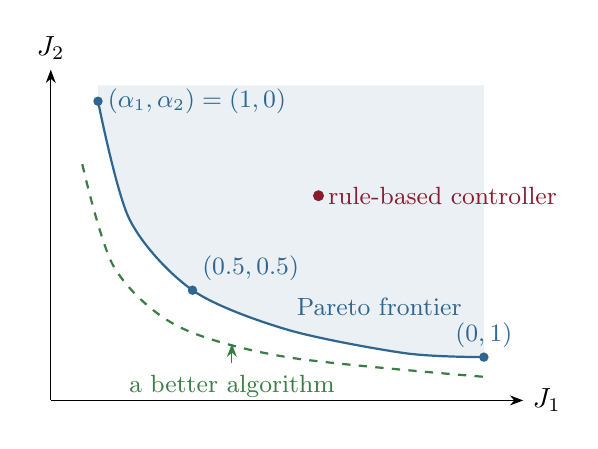
\begin{tikzpicture}[x=1cm,y=1cm,>=Stealth]
  \draw[->] (0,0) -- (6,0) node[right] {$J_1$};
  \draw[->] (0,0) -- (0,4.2) node[above] {$J_2$};
  \fill[mpc!10] plot[smooth] coordinates {(0.6,3.8) (1.0,2.3) (1.8,1.4) (3.0,0.9) (4.5,0.6) (5.5,0.55)} -- (5.5,4) -- (0.6,4) -- cycle;
  \draw[thick,mpc] plot[smooth] coordinates {(0.6,3.8) (1.0,2.3) (1.8,1.4) (3.0,0.9) (4.5,0.6) (5.5,0.55)};
  \node[mpc,font=\small,above right] at (3.0,0.95) {Pareto frontier};
  \fill[mpc] (0.6,3.8) circle (0.06) node[right,font=\small] {$(\alpha_1,\alpha_2)=(1,0)$};
  \fill[mpc] (5.5,0.55) circle (0.06) node[above,font=\small] {$(0,1)$};
  \fill[mpc] (1.8,1.4) circle (0.06) node[above right,font=\small] {$(0.5,0.5)$};
  \fill[sap] (3.4,2.6) circle (0.07) node[right,font=\small,sap] {rule-based controller};
  \draw[thick,dashed,ess] plot[smooth] coordinates {(0.4,3.0) (0.8,1.7) (1.6,0.95) (3.0,0.55) (5.5,0.3)};
  \node[ess,font=\small,anchor=north] at (2.3,0.45) {a better algorithm};
  \draw[->,ess] (2.3,0.47) -- (2.3,0.72);
\end{tikzpicture}
\caption{Two goals to minimize. The weighted sum with a given pair of weights selects one point
of the Pareto frontier; a rule-based controller lies above it; an algorithm with a larger
decision space pushes the frontier down.}
\label{fig:pareto}
\end{figure}

\subsection{The terminal value of a stored resource}

Economic problems have their own version of the terminal cost, and the building case study
(\cref{sec:building}) shows it. A controller that minimizes a bill over a window of one day
sells the energy stored in a battery before the window ends, because within the window that
sale is a profit and what happens afterwards does not exist. The behaviour is correct for the
problem written, and wrong for the application.

The remedy is to maximize the \emph{total value} over the window: the value of the state the
controller starts from, plus the profits minus the costs of what it plans, plus the value of
the state it leaves behind. The first term does not depend on the decisions, so maximizing the
total value is the same as minimizing
\begin{equation}
  J^{cost} - V(x_{\ik{N}}),
\end{equation}
where $V(x_{\ik{N}})$ is the price put on the resource still stored at the end of the window ---
for a battery, $V(x) = c^{avg}\,x$ with $c^{avg}$ the average purchase price of energy over the
day. This is the terminal cost of \cref{sec:optimality} seen from the side of the application:
it prices what happens after the horizon, and without it the controller is myopic in exactly
the way the theory predicts.

\begin{reading}
\refkey{Rawlings\_2017}, section 2.8, ``Economic Model Predictive Control'' (pp.~153--160): how
the economic problem differs from the tracking one, and which assumptions replace the positive
definite cost. \refkey{Boyd\_2004}, section 4.7, ``Vector optimization'' (pp.~174--187), in
particular 4.7.3 on Pareto optimal points and 4.7.4 on scalarization, which is the weighted sum
\eqref{eq:weighted} and the reason the weights can be normalized.
\end{reading}

\section{Writing logic as constraints}
\label{sec:toolbox}

Many decisions in the case studies are logical: a storage charges or discharges, an appliance
starts or does not, a light is green or red, a task runs on a machine or not. Optimization
solvers do not handle logic; they handle linear inequalities. This chapter collects the
constructions that translate the one into the other. Each uses \emph{binary variables},
$\delta \in \{0,1\}$, and the result is a mixed-integer linear program --- harder than a
continuous one, but far more tractable than a nonlinear one. The constructions are used
repeatedly in \cref{sec:cases}.

\subsection{Indicator variables and the big-M constraint}
\label{sec:bigM}

Let $p \ge 0$ be a continuous variable with a known upper bound $p^{\max}$, and let $\delta$ be
the binary that is meant to indicate whether $p$ is positive. The \emph{indicator constraint}
\begin{equation}
  p \le M\,\delta, \qquad M \ge p^{\max},
  \label{eq:bigM}
\end{equation}
forces $p = 0$ when $\delta = 0$ and leaves $p$ free in $[0, M]$ when $\delta = 1$. It does not
force $\delta = 1$ whenever $p > 0$ by itself; that direction is not needed when the cost makes
an unnecessary $\delta = 1$ never cheaper, which is the usual situation. The constant $M$ should
be as small as the bounds allow, $M = p^{\max}$, so that the relaxation of the problem --- the
one obtained by letting $\delta$ take values in $[0,1]$, which solvers use to guide the search
--- is as tight as possible.

\subsection{Mutually exclusive events}

Two events that cannot happen at the same time --- charging and discharging a battery, importing
and exporting power at a meter --- are written with one indicator each and the constraint
\begin{equation}
  \delta^{a} + \delta^{b} \le 1 .
\end{equation}
Combined with \eqref{eq:bigM} on each power, at most one of the two powers can be positive at a
time. The construction is what makes it possible to write a quantity with two different models
in the two cases, for instance a storage with a charging efficiency and a different discharging
efficiency:
\begin{equation}
\begin{gathered}
  p^{ess} = p^{ch} - p^{dis}, \qquad
  x_{k+1} = x_k + \eta^{ch}\,T\,p^{ch}_k - \tfrac{1}{\eta^{dis}}\,T\,p^{dis}_k, \\
  p^{ch} \le p^{ch,\max}\delta^{ch},\qquad p^{dis} \le p^{dis,\max}\delta^{dis},\qquad
  \delta^{ch} + \delta^{dis} \le 1 ,
\end{gathered}
\end{equation}
which is linear, whereas the same model written with $\max\{0,p\}$ and $\min\{0,p\}$ is not.

\subsection{Semi-continuous variables}

A device that is either off or working between a minimum and a maximum level --- a charger that
cannot deliver an arbitrarily small power --- has a \emph{semi-continuous} variable: $p = 0$ or
$p^{\min} \le p \le p^{\max}$. With one indicator the two inequalities
\begin{equation}
  \delta\,p^{\min} \;\le\; p \;\le\; \delta\,p^{\max}
  \label{eq:semicont}
\end{equation}
force $p = 0$ when $\delta = 0$ and $p \in [p^{\min}, p^{\max}]$ when $\delta = 1$.

\subsection{One start per job: one-hot variables}

A job with a known duration and a known power profile has to be executed once, inside a window
between an earliest start $S$ and a deadline $F$. The decision is \emph{when} to start it, and it
is written with one binary per admissible start time, $s_j \in \{0,1\}$ for $j = S, \dots,
F - N_{job}$, where $N_{job}$ is the duration in steps and the upper limit is the last instant
at which the job still finishes before the deadline. Exactly one of them is one:
\begin{equation}
  \sum_{j=S}^{F-N_{job}} s_j = 1 .
  \label{eq:onehot}
\end{equation}
The power of the job at time $i$ is then the profile placed where the start variable says,
\begin{equation}
  p_i = \sum_{j} s_j\, P(i - j + 1),
  \label{eq:shifted}
\end{equation}
a convolution of the profile $P(\cdot)$ with the one-hot sequence (\cref{fig:onehot}).

\begin{figure}[t]
\centering
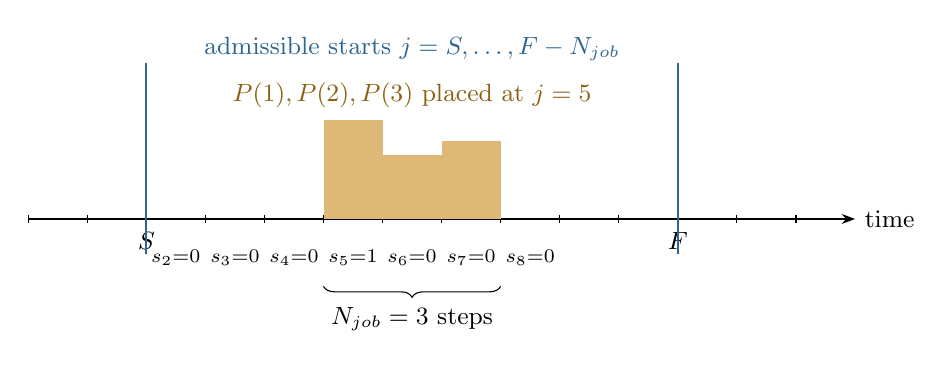
\begin{tikzpicture}[x=0.75cm,y=0.9cm,>=Stealth]
  \draw[->] (0,0) -- (14,0) node[right,font=\small] {time};
  \foreach \t in {0,...,13} \draw (\t,0.06) -- (\t,-0.06);
  \node[below,font=\small] at (2,-0.05) {$S$};
  \node[below,font=\small] at (11,-0.05) {$F$};
  \draw[mpc,thick] (2,-0.5) -- (2,2.2);
  \draw[mpc,thick] (11,-0.5) -- (11,2.2);
  \node[mpc,font=\small,above] at (6.5,2.1) {admissible starts $j = S,\dots,F-N_{job}$};
  % one-hot row
  \foreach \j/\v in {2/0,3/0,4/0,5/1,6/0,7/0,8/0} \node[font=\scriptsize] at (\j+0.5,-0.55) {$s_{\j}{=}\v$};
  % profile placed at j=5
  \fill[sun!60] (5,0) rectangle (6,1.4);
  \fill[sun!60] (6,0) rectangle (7,0.9);
  \fill[sun!60] (7,0) rectangle (8,1.1);
  \node[sun!70!black,font=\small] at (6.5,1.75) {$P(1),P(2),P(3)$ placed at $j=5$};
  \draw[decorate,decoration={brace,amplitude=4pt,mirror}] (5,-0.95) -- (8,-0.95) node[midway,below=4pt,font=\small] {$N_{job}=3$ steps};
\end{tikzpicture}
\caption{Load shifting with one-hot start variables. Exactly one $s_j$ equals one inside the
admissible range, and the power profile of the job is placed at that start.}
\label{fig:onehot}
\end{figure}

\subsection{The product of a real variable and a binary}
\label{sec:product}

A term $q\,b$, with $q \in [\underline q, \bar q]$ real and $b \in \{0,1\}$, is not linear. It
is replaced by a new variable $p$ and two pairs of inequalities:
\begin{equation}
  \underline q\, b \le p \le \bar q\, b, \qquad
  q - M(1-b) \le p \le q + M(1-b), \qquad M \ge \max\{\abs{\underline q}, \abs{\bar q}\} .
  \label{eq:product}
\end{equation}
When $b = 0$ the first pair forces $p = 0$ and the second says nothing; when $b = 1$ the second
pair forces $p = q$ and the first is vacuous. The construction recurs in every formulation with
timers, such as the duration of a traffic-light colour, $t_{i+1} = (t_i + T)\,y_i$.

\subsection{Maxima and absolute values}

A goal of the form ``minimize the largest of several quantities'' is not a sum. It is handled
with an \emph{epigraph} variable: to minimize $\max_v w_v$ over a set of quantities $w_v$,
introduce $\bar w$ with the constraints $w_v \le \bar w$ for every $v$, and minimize $\bar w$.
The bound is pushed down until it rests on the largest $w_v$. The same device writes an
absolute value in a cost: $\abs{x}$ is replaced by $x^{+} + x^{-}$ with $x = x^{+} - x^{-}$,
$x^{+}, x^{-} \ge 0$, exact as long as the cost is increasing in both; this is how a tracking
error $\abs{P - P^{ref}}$ enters a linear program. A convex piecewise-linear cost, such as an
approximation of a square, is written in the same way with several pieces of increasing price.

\subsection{Soft constraints and slack variables}
\label{sec:soft}

A constraint that may be impossible to satisfy --- a deadline for a charge when the vehicle
arrives too late, a stop requested in the only hours in which a load can run --- must not be
written as a hard constraint, or the problem becomes infeasible and the controller has nothing
to apply. It is \emph{relaxed} with a non-negative slack variable that measures the violation,
and the violation is paid for in the cost:
\begin{equation}
  g(x) \le 0 \quad\longrightarrow\quad g(x) \le \varepsilon,\ \ \varepsilon \ge 0,
  \qquad J \leftarrow J + d\,\varepsilon \ \text{ or } \ J + d\,\varepsilon^2 .
  \label{eq:slack}
\end{equation}
The weight $d$ sets the behaviour: small, and the controller violates the constraint when that
improves the other goals; large, and it violates it only when the constraint cannot be met at
all. With several relaxed constraints the quadratic form $\sum_p \varepsilon_p^2$ is preferable
to the linear one, because it prefers many small violations to one large one --- it is fairer.

\begin{reading}
\refkey{Hax\_1977}, chapter 9, for integer programming and the modelling of logical conditions:
indicator variables, big-M, mutually exclusive alternatives, fixed charges.
\refkey{Borrelli\_2017} for the same constructions inside an MPC problem, in the framework of
mixed logical dynamical systems. \refkey{Boyd\_2004}, section 4.1.3, for the epigraph form of an
optimization problem.
\end{reading}

\section{Case studies}
\label{sec:cases}

The case studies follow the same pattern. The control goals are identified; they are turned
into a cost; the system is modelled with states, inputs and disturbances; the limits of the
system and the logic of the application become constraints; and the resulting problem is solved
at every step on a receding horizon. All of them are economic MPC problems in the sense of
\cref{sec:economic}, and all use the constructions of \cref{sec:toolbox}. For each of them the
course website has an interactive laboratory that runs the controller in the browser.

\subsection{The charging service area}
\label{sec:servicearea}

\paragraph{Problem.} A service area for the fast charging of electric vehicles draws power from
the grid at a point of connection (POC). Vehicles arrive wanting to recharge as fast as
possible, so even a few of them produce a large power flow, which means a large connection and
a heavy bill under a capacity-based tariff. An energy storage system (ESS) is installed to keep
the power at the point of connection small. On site there may also be a renewable generator.

\paragraph{Variables and model.} With the \emph{consumer sign convention} --- power consumed is
positive --- the quantities at time $i$ of the window opened at $k$ are: the charging demand of
the vehicles $p^{pev}_{\ik{i}}$ and the renewable generation $p^{res}_{\ik{i}}$, both known over
the window (disturbances with a forecast); the storage power $u_{\ik{i}}$, positive when
charging, which is the control; the energy stored $x_{\ik{i}}$, which is the state; and the power
at the point of connection $p_{\ik{i}}$, which is the controlled quantity. The balance at the
point of connection and the dynamics of the storage are
\begin{equation}
  p_{\ik{i}} = p^{pev}_{\ik{i}} + u_{\ik{i}} - p^{res}_{\ik{i}}, \qquad
  x_{\ik{i+1}} = x_{\ik{i}} + \tfrac{T}{3600}\, u_{\ik{i}}, \qquad x_{\ik{0}} = x_k .
\end{equation}

\paragraph{Problem solved at every step.}
\begin{equation}
\begin{aligned}
  \min_{u} \quad & \sum_{i=0}^{N-1}\Big[\alpha\, p_{\ik{i}}^2 + \beta\,\big(x_{\ik{i}} - x^{ref}\big)^2\Big]
                   + \beta_f\,\big(x_{\ik{N}} - x^{ref}\big)^2 \\
  \st \quad & \text{balance, dynamics, } x_{\ik{0}} = x_k, \\
            & u^{\min} \le u_{\ik{i}} \le u^{\max},\quad x^{\min} \le x_{\ik{i}} \le x^{\max},\quad
              p^{\min} \le p_{\ik{i}} \le p^{\max}.
\end{aligned}
\end{equation}
The weight $\alpha$ penalizes the power at the point of connection; $\beta$, deliberately
small, keeps the storage near a reference level so that it is ready for the next event; the
terminal weight $\beta_f$ is taken from the Riccati equation of the unconstrained problem, as
\cref{sec:optimality} prescribes. Since $p$ is an affine function of $u$, the limits on $p$ are
bounds on the control, and the problem is a quadratic program.

\paragraph{Losses and indicators.} A real storage has a charging and a discharging efficiency,
and the two cases obey different equations. The storage power is split into a charging and a
discharging power, $p^{ess} = p^{ch} - p^{dis}$, both non-negative, with the indicator variables
$\delta^{ch}, \delta^{dis}$, the constraints $p^{ch} \le p^{ch,\max}\delta^{ch}$, $p^{dis} \le
p^{dis,\max}\delta^{dis}$, $\delta^{ch} + \delta^{dis} \le 1$, and the dynamics with the
efficiencies, as in \cref{sec:toolbox}. The problem becomes a mixed-integer quadratic program.
We also distinguished the \emph{control model}, which lives inside the MPC problem and is the
controller's belief about the plant, from the \emph{simulation model}, which replaces the real
system when the controller is tested.

\paragraph{Code.} The implementation is split in two files on purpose: \texttt{main.jl} is the
application, which holds the parameters, builds the profiles and runs the receding-horizon loop
--- measure, call the optimizer, apply the first control, simulate one step, repeat;
\texttt{MPC\_iteration.jl} is the controller, which builds the optimization problem in the
modelling language JuMP and hands it to a solver. Changing solver is one line, and the model
does not change: this separation between how a problem is written and how it is solved is the
reason for using a modelling language at all.

\begin{labbox}
The Service Area Lab runs the controller over a full day against the same area without storage;
the peak at the point of connection halves. The lab also shows the effect of the horizon, of the
forecast, and of the terminal weight. The Julia code of the lesson is on the website, with the
formulation it implements. Among real installations, battery-buffered fast chargers sold for
sites with a weak grid connection are this problem turned into a product.
\end{labbox}

\subsection{Building energy management}
\label{sec:building}

\paragraph{Problem.} A building has photovoltaic panels, non-plannable loads, plannable loads,
an energy storage system and a charging station, all behind one meter at the point of delivery
(\cref{fig:building}). The first goal is to minimize the electricity bill under a time-of-use
tariff, with one price $c^{in}$ for the energy consumed and a lower price $c^{out}$ for the
energy injected into the grid.

\begin{figure}[t]
\centering
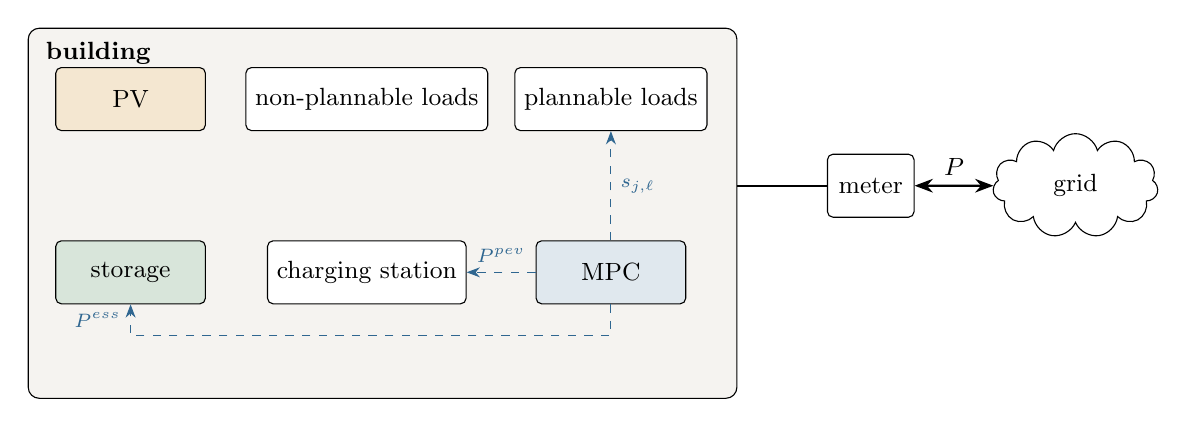
\begin{tikzpicture}[x=1cm,y=1cm,>=Stealth,
  box/.style={draw,rounded corners=2pt,minimum width=1.9cm,minimum height=0.8cm,font=\small,fill=white}]
  \draw[rounded corners=4pt,fill=soft] (-0.4,-1.1) rectangle (8.6,3.6);
  \node[font=\small\bfseries,anchor=north west] at (-0.3,3.55) {building};
  \node[box,fill=sun!20] (pv) at (0.9,2.7) {PV};
  \node[box] (npl) at (3.9,2.7) {non-plannable loads};
  \node[box] (pl) at (7.0,2.7) {plannable loads};
  \node[box,fill=ess!20] (ess) at (0.9,0.5) {storage};
  \node[box] (cs) at (3.9,0.5) {charging station};
  \node[box,fill=mpc!15] (mpc) at (7.0,0.5) {MPC};
  \node[box,minimum width=1.1cm] (meter) at (10.3,1.6) {meter};
  \node[draw,cloud,cloud puffs=11,minimum width=2.1cm,minimum height=1.3cm,font=\small] (grid) at (12.9,1.6) {grid};
  \draw[thick] (8.6,1.6) -- (meter);
  \draw[thick,<->] (meter) -- (grid) node[midway,above,font=\small] {$P$};
  \draw[dashed,mpc,->] (mpc.south) -- ++(0,-0.4) -| (ess.south) node[pos=0.75,left,font=\scriptsize,mpc] {$P^{ess}$};
  \draw[dashed,mpc,->] (mpc) -- (cs) node[midway,above,font=\scriptsize,mpc] {$P^{pev}$};
  \draw[dashed,mpc,->] (mpc) -- (pl) node[midway,right,font=\scriptsize,mpc] {$s_{j,\ell}$};
\end{tikzpicture}
\caption{The building of the second case study. The controller acts on the storage, on the
charging station and on the start times of the plannable loads; generation and non-plannable
loads are forecasts; the bill is paid on the power at the meter.}
\label{fig:building}
\end{figure}

\paragraph{Plannable loads.} Each plannable load $\ell$ comes with the preferences of the user,
the earliest start $S_\ell$, the deadline $F_\ell$, the duration $N_\ell$, and with its power
profile $P_\ell$. Load shifting is the decision of when to start it, written with the one-hot
variables $s_{\ik{j},\ell}$ of \cref{sec:toolbox}: the load starts exactly once,
$\sum_{j=S_\ell}^{F_\ell - N_\ell} s_{\ik{j},\ell} = 1$, its power is the shifted profile
$P^{pl}_{\ik{i},\ell} = \sum_j s_{\ik{j},\ell}\,P_\ell(i-j+1)$, and the total plannable power is
$P^{pl}_{\ik{i}} = \sum_\ell P^{pl}_{\ik{i},\ell}$. Note the two time indices: $S_\ell$ and
$F_\ell$ are absolute times, $i|k$ is relative to the window.

\paragraph{The bill.} The power at the meter, $P_{\ik{i}} = P^{npl} + P^{pl} + P^{pev} + P^{ess}
- P^{pv}$, is a cost when positive and a revenue when negative. It is split as $P = P^{in} -
P^{out}$ with $P^{in}, P^{out} \ge 0$, the two forbidden from being positive together by the
indicators $\delta^{in}, \delta^{out}$ and the constraints $P^{in} \le P^{\max}\delta^{in}$,
$P^{out} \le \abs{P^{\min}}\delta^{out}$, $\delta^{in} + \delta^{out} \le 1$. The bill over the
window is then linear:
\begin{equation}
  J^{cost} = \sum_{i=0}^{N-1} \tfrac{T}{3600}\Big(c^{in}_{\ik{i}} P^{in}_{\ik{i}} - c^{out}_{\ik{i}} P^{out}_{\ik{i}}\Big).
\end{equation}

\paragraph{Battery ageing.} A storage system has a price $COST^{ess}$ and a finite number of
full cycles. The energy it will move over its life is $E^{life} = 2\,x^{ess,\max}\cdot
\mathit{cycles}$, and the ratio $c^{dep} = COST^{ess}/E^{life}$ is what one kWh through the
battery costs in terms of life consumed --- a few cents. Both charging and discharging consume
life, so the term is
\begin{equation}
  J^{depr} = \sum_{i=0}^{N-1} c^{dep}\,\big(P^{ch}_{\ik{i}} + P^{dis}_{\ik{i}}\big)\,\tfrac{T}{3600},
\end{equation}
which is $c^{dep}\abs{P^{ess}}$ written without an absolute value, thanks to the split into two
non-negative powers. It acts as a friction: the storage is used only when the benefit exceeds
the loss of life.

\paragraph{The full objective.} With a regulation term on the stored energy and the terminal
value of \cref{sec:economic},
\begin{equation}
  J = J^{cost} + \alpha_x \sum_{i}\big(x^{ess}_{\ik{i}} - x^{ref}\big)^2 + \alpha_{dep}\,J^{depr}
      - c^{avg}\,x^{ess}_{\ik{N}} ,
\end{equation}
subject to the balance at the meter, the dynamics of the storage with its efficiencies, the
measured initial state, the one-hot constraints of the loads, the indicator constraints and the
bounds on all variables. Without the last term the battery ends every day empty, because selling
its energy is a profit inside the window; with it, the energy left is valued at the average
purchase price and the controller keeps it. The weights are chosen as in \cref{sec:economic},
and they can be normalized to sum to one.

\paragraph{What was left out.} The model is electrical only. A real battery management system
also tracks the state of charge in percent, the state of health, which cell balancing protects,
and the state of power, the power the battery can deliver in the near future. The thermal part
of the building --- wall and room temperatures driven by the weather and by heating and
cooling, humidity, air quality, ventilation --- would add comfort terms to the objective and
constraints of its own. The building information model is the source from which the parameters
of all these models can be updated as the building changes.

\begin{labbox}
The Building Energy Lab runs this problem on a detached house with five appliances under a
time-of-use tariff, and compares the plan with an uncontrolled house and with a rule-based
battery. Two experiments belong to this chapter: removing the terminal value and watching the
battery end the day empty, and asking the house for a flexibility service --- a power cap or a
power curve --- with a fee for delivering it and a penalty for failing. Measured
demonstrations of predictive control on real buildings exist, on offices, with savings of the
order of tens of percent on the energy for heating and cooling.
\end{labbox}

\subsection{An aggregator of electric vehicles}
\label{sec:aggregator}

\paragraph{Context.} Electricity is traded on wholesale markets by generators, retailers and
the market operator. Next to them, the transmission and distribution system operators buy on
the \emph{ancillary services} or \emph{flexibility} markets what they need to keep frequency
and voltage at their references. The providers are large consumers or \emph{aggregators} of
many small resources, managed as one entity to reach the minimum bidding size --- of the order
of a megawatt for a given window. A fleet of charging vehicles is such an aggregation: the goal
of the aggregator is to make the \emph{total} charging power of the fleet track a profile agreed
with the market, while every driver still receives the charge requested.

\paragraph{Model.} For each vehicle $p$ connected during the window, a charging and a
discharging power, $P^{ch}_{\ik{i},p}, P^{dis}_{\ik{i},p} \ge 0$, with their indicators and
mutual exclusion; the stored energy with the efficiencies,
$x_{\ik{i+1},p} = x_{\ik{i},p} + \eta^{ch}\,T\,P^{ch}_{\ik{i},p} - \tfrac{1}{\eta^{dis}}\,T\,P^{dis}_{\ik{i},p}$;
and the fact that a charger cannot deliver an arbitrarily small power, the semi-continuous
constraint \eqref{eq:semicont}, $\delta^{ch}_{\ik{i},p}P^{ch,\min}_p \le P^{ch}_{\ik{i},p} \le
\delta^{ch}_{\ik{i},p}P^{\max}_p$. The total power is $P_{\ik{i}} = \sum_p \big(P^{ch}_{\ik{i},p}
- P^{dis}_{\ik{i},p}\big)$.

\paragraph{User preferences.} Each driver states a final charging time $F_p$ and a desired
state of charge $x^{ref}_p$. If the vehicle leaves inside the window, $F_p \le k + N$, the
request is a constraint, $x_{F_p|k,p} \ge x^{ref}_p$; if it leaves after the window, the request
enters the cost as a term $(x_{\ik{N},p} - x^{ref}_p)^2$. The constraint can be impossible to
meet --- a vehicle that arrives too empty or stays too little --- and it is therefore
\emph{relaxed} as in \cref{sec:soft}:
\begin{equation}
  x_{F_p|k,p} \ge x^{ref}_p - \varepsilon_p, \qquad \varepsilon_p \ge 0 .
\end{equation}

\paragraph{Objective.}
\begin{equation}
  J = d_1 \sum_{i=0}^{N-1}\big(P_{\ik{i}} - P^{ref}_{\ik{i}}\big)^2
    + d_2 \sum_{p:\,F_p > k+N}\big(x_{\ik{N},p} - x^{ref}_p\big)^2
    + d_3 \sum_{p} \varepsilon_p^2 .
\end{equation}
The weight $d_3$ decides the behaviour: small, and the controller disappoints a driver to follow
the grid better; large, and it disappoints a driver only when the request cannot be met at all.
Sweeping it traces the Pareto frontier between the two goals.

\begin{labbox}
The PEV Aggregator Lab runs the problem in closed loop over a day, with the request for a stop
in the aggregate power arriving at a chosen hour: until then the controller spreads the charge,
and at that hour the plan is rearranged. In Italy the role described here is regulated: Terna's
UVAM pilot admits aggregates of loads, storage and vehicles of at least one megawatt into the
balancing market, paid for availability and for the energy actually moved.
\end{labbox}

\subsection{Traffic lights at an intersection}
\label{sec:traffic}

\paragraph{Problem.} One intersection with a set $\mathcal{J}$ of traffic lights, one per
approaching road (\cref{fig:intersection}). Two goals belong to two different people: the
traffic manager wants short queues, the drivers want short waiting times.

\begin{figure}[t]
\centering
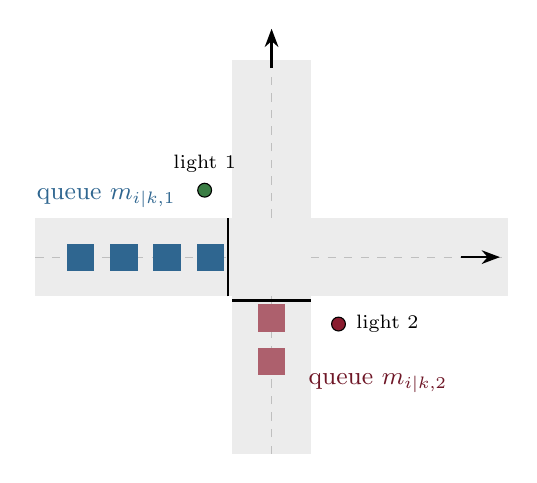
\begin{tikzpicture}[x=1cm,y=1cm,>=Stealth]
  \fill[gray!15] (-3,-0.5) rectangle (3,0.5);
  \fill[gray!15] (-0.5,-2.5) rectangle (0.5,2.5);
  \draw[gray!50,dashed] (-3,0) -- (-0.5,0);
  \draw[gray!50,dashed] (0.5,0) -- (3,0);
  \draw[gray!50,dashed] (0,-2.5) -- (0,-0.5);
  \draw[gray!50,dashed] (0,0.5) -- (0,2.5);
  \draw[thick] (-0.55,-0.5) -- (-0.55,0.5);
  \draw[thick] (-0.5,-0.55) -- (0.5,-0.55);
  \foreach \i in {0,...,3} \fill[mpc] (-0.95-0.55*\i,-0.17) rectangle (-0.6-0.55*\i,0.17);
  \foreach \i in {0,1} \fill[sap!70] (-0.17,-0.95-0.55*\i) rectangle (0.17,-0.6-0.55*\i);
  \node[font=\small,mpc] at (-2.1,0.75) {queue $m_{\ik{i},1}$};
  \node[font=\small,sap!80!black] at (1.35,-1.6) {queue $m_{\ik{i},2}$};
  \draw[->,thick] (2.4,0) -- (2.9,0);
  \draw[->,thick] (0,2.4) -- (0,2.9);
  \node[circle,draw,fill=ess,minimum size=5pt,inner sep=0] at (-0.85,0.85) {};
  \node[font=\scriptsize,above] at (-0.85,0.95) {light 1};
  \node[circle,draw,fill=sap,minimum size=5pt,inner sep=0] at (0.85,-0.85) {};
  \node[font=\scriptsize,right] at (0.95,-0.85) {light 2};
\end{tikzpicture}
\caption{The intersection of the fourth case study: two one-way roads, one light each, queues
counted at the stop lines.}
\label{fig:intersection}
\end{figure}

\paragraph{Control variables.} The colours: for each light $J$ three binaries
$g_{\ik{i},J}, y_{\ik{i},J}, r_{\ik{i},J} \in \{0,1\}$, exactly one of which is on,
\begin{equation}
  g_{\ik{i},J} + y_{\ik{i},J} + r_{\ik{i},J} = 1 .
\end{equation}
The admissible transitions are green $\to$ yellow $\to$ red $\to$ green, and each forbidden
transition is a linear inequality: green cannot be followed by red, red by yellow, yellow by
green,
\begin{equation}
  r_{\ik{i+1},J} \le 1 - g_{\ik{i},J}, \qquad
  y_{\ik{i+1},J} \le 1 - r_{\ik{i},J}, \qquad
  g_{\ik{i+1},J} \le 1 - y_{\ik{i},J}.
\end{equation}
The same inequalities, written between the first step of the window and the colour actually
displayed at $k-1$, tie the plan to the current state of the lights. Conflicting lights cannot
be green or yellow at the same time, $\sum_{J}\big(g_{\ik{i},J} + y_{\ik{i},J}\big) \le 1$.

\paragraph{The yellow.} Safety requires a minimum duration of the yellow. A timer counts how
long the yellow has been on, $t^y_{\ik{i+1},J} = (t^y_{\ik{i},J} + T)\,y_{\ik{i},J}$, a product
of a real variable and a binary linearized as in \cref{sec:product}, and the light cannot turn
red before the timer reaches the minimum:
\begin{equation}
  r_{\ik{i+1},J} \le \frac{t^y_{\ik{i},J}}{t^{y,\min}_J} + \big(1 - y_{\ik{i},J}\big).
\end{equation}
While the timer is short of the minimum the first term is strictly less than one, and since
$r$ is binary the constraint forces $r_{\ik{i+1},J} = 0$; the second term makes the constraint
irrelevant when the light is not yellow.

\paragraph{Queues and waiting times.} Two models. The \emph{aggregate} model keeps one state
per light, the number of vehicles waiting, with the dynamics
\begin{equation}
  m_{\ik{i+1},J} = m_{\ik{i},J} + v^{in}_{\ik{i},J}\,T - v^{out}_{J}\,T\,g_{\ik{i},J},
  \qquad m_{\ik{0},J} = m_{k,J} \text{ measured},\quad m \ge 0,
\end{equation}
where $v^{in}$ is the arrival rate and $v^{out}$ the discharge rate on green; the constraint
$m \ge 0$ is an approximation of the fact that a queue cannot become negative. Average waiting
times then follow from Little's law. The \emph{detailed} model keeps position, speed and
acceleration of every vehicle, the acceleration being a model of the driver for human-driven
cars and a command for automated ones, and a binary $\delta_{\ik{i},v}$ that says whether the
vehicle is still in the queue, so that its waiting time grows as $w_{\ik{i+1},v} = (w_{\ik{i},v}
+ T)\,\delta_{\ik{i},v}$ and the queue length is the sum of the indicators.

\paragraph{Objective.} On the queues, $J^m = \sum_i \sum_J m_{\ik{i},J}^2$: the square
shortens the queues and balances them, since for a given total it prefers two queues of five
to one of ten. On the waiting times the goal is to minimize the \emph{largest} of them, written
with an epigraph variable $\bar w_{\ik{i}}$, $w_{\ik{i},v} \le \bar w_{\ik{i}}$ for every vehicle
present, and $J^w = \sum_i \bar w_{\ik{i}}^2$ in the cost. The problem is a mixed-integer
quadratic program; a city is many intersections tied by coupling constraints, which is where
centralized and distributed MPC return.

\begin{labbox}
The Traffic Light Lab runs the intersection of \cref{fig:intersection} with the same vehicles
arriving on both sides of the screen, a fixed-time plan on the left and the MPC on the right,
with queues and waiting times compared as the day goes on. With two lights the transition
constraints leave few enough admissible colour sequences over the window for the page to
enumerate them and find the best one exactly; the mixed-integer formulation is what is needed
when the intersection is larger. Systems of this kind run in cities: Surtrac in Pittsburgh re-plans every intersection on
a rolling horizon about once a second, and UTOPIA, born in Turin, has been in operation since
the nineteen-eighties.
\end{labbox}

\subsection{Task scheduling in an assembly line}
\label{sec:scheduling}

\emph{This section covers what was done in class up to the lesson of 26 October; it will be
completed after the next lesson.}

\paragraph{Problem.} A \emph{job} --- the assembly of a vehicle --- is made of elementary
\emph{tasks}, executed on \emph{workstations} and requiring \emph{resources}: tools, people,
energy. Among the possible goals --- cost, quality, scrap, balanced use of the workstations ---
the one taken here is the total completion time of the job, the \emph{makespan}, read on a
Gantt chart. The orders of magnitude are what makes the problem hard: ten thousand tasks over
sixty days.

\paragraph{Sets and parameters.} The tasks $\mathcal{T}$, the workstations $\mathcal{W}$ and,
for each task, the subset $\mathcal{W}_t \subseteq \mathcal{W}$ of workstations that can execute
it. Each task $t$ carries an earliest start $S_t$, a deadline $F_t$, an estimate $d_t$ of the
number of steps it needs, and the number $R^{\#}_{t,r}$ of resources of each type $r \in
\mathcal{R}$ it consumes; $R^{a}_r$ is the number available.

\paragraph{Decision variables and dynamics.} One binary per task, workstation and time,
$e_{\ik{i},t,w} \in \{0,1\}$, equal to one when task $t$ runs at time $i|k$ on workstation $w$.
A task runs on at most one workstation at a time,
\begin{equation}
  \sum_{w \in \mathcal{W}_t} e_{\ik{i},t,w} \le 1, \qquad
  e_{\ik{i},t} = \sum_{w \in \mathcal{W}_t} e_{\ik{i},t,w} \in \{0,1\},
\end{equation}
where the auxiliary $e_{\ik{i},t}$ says whether the task is running. The state is the time left
to complete each task, decremented by one unit for every step actually worked,
\begin{equation}
  d_{\ik{i+1},t} = d_{\ik{i},t} - \sum_{w \in \mathcal{W}_t} e_{\ik{i},t,w},
\end{equation}
and the deadline is $d_{F_t,t} = 0$ for every task whose deadline falls inside the window.

\paragraph{Precedence constraints.} The relations that make a schedule a schedule:
finish-to-start, finish-to-finish, start-to-start, start-to-finish. The first, task $t_2$ cannot
run until $t_1$ is finished, is the one to be written as an inequality in the next lesson,
together with the resource constraints and the objective.

\begin{reading}
For the modelling constructions of all five case studies, \refkey{Hax\_1977}, chapter 9, and
\refkey{Borrelli\_2017}. For the market context of the aggregator, \refkey{Kirschen\_2019},
chapter 3 on markets for electrical energy and chapter 6 on power system operation; background
reading. For the traffic and the scheduling applications, the papers \refkey{Liberati\_2025a}
and \refkey{Liberati\_2025b} show the same formulations on real problems; background reading,
not examination material.
\end{reading}

\clearpage
\section*{References}
\addcontentsline{toc}{section}{References}

The keys are the same as on the course website, where the links are kept up to date.

\begin{description}[style=nextline,leftmargin=0pt,labelsep=0pt,itemsep=4pt]
  \item[\refkey{Cannon\_2016}] B.~Kouvaritakis, M.~Cannon. \emph{Model Predictive Control:
    Classical, Robust and Stochastic}. Springer, 2016. Main reference of the course: chapter 2
    follows the same route, and the same notation, as these notes.
  \item[\refkey{Rawlings\_2017}] J.~B.~Rawlings, D.~Q.~Mayne, M.~Diehl. \emph{Model Predictive
    Control: Theory, Computation, and Design}, 2nd ed. Nob Hill Publishing, 2017. Free PDF from
    the authors.
  \item[\refkey{Borrelli\_2017}] F.~Borrelli, A.~Bemporad, M.~Morari. \emph{Predictive Control for
    Linear and Hybrid Systems}. Cambridge University Press, 2017.
  \item[\refkey{Boyd\_2004}] S.~Boyd, L.~Vandenberghe. \emph{Convex Optimization}. Cambridge
    University Press, 2004. Free PDF from the authors.
  \item[\refkey{Hax\_1977}] S.~P.~Bradley, A.~C.~Hax, T.~L.~Magnanti. \emph{Applied Mathematical
    Programming}. Addison-Wesley, 1977. Chapter 9.
  \item[\refkey{Kirschen\_2019}] D.~S.~Kirschen, G.~Strbac. \emph{Fundamentals of Power System
    Economics}, 2nd ed. Wiley, 2019.
  \item[\refkey{Mayne\_2000}] D.~Q.~Mayne, J.~B.~Rawlings, C.~V.~Rao, P.~O.~M.~Scokaert.
    ``Constrained model predictive control: Stability and optimality.'' \emph{Automatica} 36(6),
    789--814, 2000.
  \item[\refkey{Liberati\_2025a}] F.~Liberati, M.~Donsante, A.~Tortorelli. ``Single intersection
    MPC traffic signal control in presence of automated vehicles.'' \emph{IEEE Transactions on
    Control Systems Technology} 33(4), 1432--1446, 2025.
  \item[\refkey{Liberati\_2025b}] F.~Liberati, M.~Donsante, C.~M.~F.~Cirino, A.~Tortorelli. ``Fast
    task scheduling with model predictive control integrating a priority-based heuristic.''
    \emph{IEEE Access} 13, 14499--14515, 2025.
\end{description}


\end{document}
